% Options for packages loaded elsewhere
\PassOptionsToPackage{unicode}{hyperref}
\PassOptionsToPackage{hyphens}{url}
%
\documentclass[
]{journal}
\title{Managing Interoperability of Healthcare Data for Decision Analytics and Research}
\author{JR Campbell, JC McClay, CR Geary, WS Campbell, \& AJ Anzalone}
\date{Tuesday, May 24, 2022 8:00 AM - 12:30 PM CDT}

\usepackage{amsmath,amssymb}
\usepackage{lmodern}
\usepackage{iftex}
\ifPDFTeX
  \usepackage[T1]{fontenc}
  \usepackage[utf8]{inputenc}
  \usepackage{textcomp} % provide euro and other symbols
\else % if luatex or xetex
  \usepackage{unicode-math}
  \defaultfontfeatures{Scale=MatchLowercase}
  \defaultfontfeatures[\rmfamily]{Ligatures=TeX,Scale=1}
\fi
% Use upquote if available, for straight quotes in verbatim environments
\IfFileExists{upquote.sty}{\usepackage{upquote}}{}
\IfFileExists{microtype.sty}{% use microtype if available
  \usepackage[]{microtype}
  \UseMicrotypeSet[protrusion]{basicmath} % disable protrusion for tt fonts
}{}
\makeatletter
\@ifundefined{KOMAClassName}{% if non-KOMA class
  \IfFileExists{parskip.sty}{%
    \usepackage{parskip}
  }{% else
    \setlength{\parindent}{0pt}
    \setlength{\parskip}{6pt plus 2pt minus 1pt}}
}{% if KOMA class
  \KOMAoptions{parskip=half}}
\makeatother
\usepackage{xcolor}
\IfFileExists{xurl.sty}{\usepackage{xurl}}{} % add URL line breaks if available
\IfFileExists{bookmark.sty}{\usepackage{bookmark}}{\usepackage{hyperref}}
\hypersetup{
  pdftitle={Managing Interoperability of Healthcare Data for Decision Analytics and Research},
  pdfauthor={JR Campbell, JC McClay, CR Geary, WS Campbell, \& AJ Anzalone},
  hidelinks,
  pdfcreator={LaTeX via pandoc}}
\urlstyle{same} % disable monospaced font for URLs
\usepackage{longtable,booktabs,array}
\usepackage{calc} % for calculating minipage widths
% Correct order of tables after \paragraph or \subparagraph
\usepackage{etoolbox}
\makeatletter
\patchcmd\longtable{\par}{\if@noskipsec\mbox{}\fi\par}{}{}
\makeatother
% Allow footnotes in longtable head/foot
\IfFileExists{footnotehyper.sty}{\usepackage{footnotehyper}}{\usepackage{footnote}}
\makesavenoteenv{longtable}
\usepackage{graphicx}
\makeatletter
\def\maxwidth{\ifdim\Gin@nat@width>\linewidth\linewidth\else\Gin@nat@width\fi}
\def\maxheight{\ifdim\Gin@nat@height>\textheight\textheight\else\Gin@nat@height\fi}
\makeatother
% Scale images if necessary, so that they will not overflow the page
% margins by default, and it is still possible to overwrite the defaults
% using explicit options in \includegraphics[width, height, ...]{}
\setkeys{Gin}{width=\maxwidth,height=\maxheight,keepaspectratio}
% Set default figure placement to htbp
\makeatletter
\def\fps@figure{htbp}
\makeatother
\setlength{\emergencystretch}{3em} % prevent overfull lines
\providecommand{\tightlist}{%
  \setlength{\itemsep}{0pt}\setlength{\parskip}{0pt}}
\setcounter{secnumdepth}{5}
\usepackage{booktabs}
\ifLuaTeX
  \usepackage{selnolig}  % disable illegal ligatures
\fi
\usepackage[]{natbib}
\bibliographystyle{plainnat}

\begin{document}
\maketitle

{
\setcounter{tocdepth}{2}
\tableofcontents
}
\hypertarget{introduction}{%
\section{Introduction}\label{introduction}}

This four-hour workshop for the advanced participant will promote interoperability and analytics in healthcare datamarts being developed and implemented for decision support, research and public health. It will guide the participant in implementing the guidelines of the ONC Interoperability Standards Advisory(ISA). The workshop team will employ their research and experience with HL7 and SNOMED CT to demonstrate the integration of SNOMED CT, LOINC and RxNORM as domain ontologies integrated with FHIR resources. Using a series of use cases taken from implementation of research network datamarts, they will present and discuss the relevant ISA specifications, and the associated ontology standards, some being developed at Nebraska. For each use case they will highlight any ambiguities in the ONC specifications and discuss the decisions to be made relative to deploying the semantics of the reference domain standards. They will present resources for managing and implementing relevant ONC sanctioned ontologies within the ISA model, including an integrated ontology of SNOMED-LOINC-RXNORM developed and published as terminology resources by Nebraska. Special attention will be focused on addressing problem areas of translational research that require integration of reference domain standards to bridge laboratory medicine, pathology, microbiology, genomics and patient phenomics. Each use case will be accompanied by demonstration of the data analytic utility of ontologies for extraction of meaningful knowledge from the EHR. Participants will conclude the workshop with an understanding of and access to a set of open source resources and tools for binding, integrating and maintaining the ontologies at their own institutions.

\hypertarget{learning-objectives}{%
\subsection{Learning Objectives}\label{learning-objectives}}

After participating in this session the learner should be better able to:

\begin{itemize}
\item
  Describe and discuss features of an interoperable data model compliant with the 2021 ONC Interoperability Standards Advisory for EHR core data domains
\item
  Understand the semantic scope, strengths and weaknesses and tooling for terminology standards: SNOMED CT, LOINC, RxNorm, NDC, (CPT-4, ICD-10-CM/PCS, CVX)
\item
  Identify and manage knowledge gaps present in domain ontologies in support logical integration of ontologies
\item
  List resources and tools of use in deploying, maintaining and updating ONC interoperability standards
\end{itemize}

\hypertarget{how-to-use-this-pamphlet}{%
\subsection{How to Use this Pamphlet}\label{how-to-use-this-pamphlet}}

This accompanying pamphlet contains references and resources that accompany the sections of this workshop. We have compiled a list of important resources on the management and maintenance of medical terminology and other measures that are available for use during and following the workshop in the \href{https://github.com/UNMC-CRANE/AMIA_Workshop_May_2022/tree/main/Handouts}{handouts folders}.

\hypertarget{handouts-inventory}{%
\subsubsection{Handouts Inventory}\label{handouts-inventory}}

\begin{itemize}
\tightlist
\item
  \href{https://github.com/UNMC-CRANE/AMIA_Workshop_May_2022/blob/main/Handouts/RUCA2010ZIPCODE.csv}{RUCA2010ZIPCODE.csv}

  \begin{itemize}
  \tightlist
  \item
    \href{https://ers.usda.gov/data-products/rural-urban-commuting-area-codes/}{2010 Rural-Urban Commuting Area (RUCA) Codes for the US organized by 5 digit zip code}.\\
    \strut \\
  \end{itemize}
\item
  \href{https://github.com/UNMC-CRANE/AMIA_Workshop_May_2022/blob/main/Handouts/RXNORM_NDC_RELATIONSHIPS_20220501.zip}{RXNORM\_NDC\_RELATIONSHIPS\_20220501.zip}

  \begin{itemize}
  \tightlist
  \item
    Comprehensive and historically complete file of useful relationships which have been published by NLM and the FDA. This includes relationships for RXCUIs, NDCs and VA Drug Classes that might now be listed as inactive in current UMLS releases. The Relationship types included are:

    \begin{enumerate}
    \def\labelenumi{\arabic{enumi})}
    \tightlist
    \item
      VA Class to Ingredient,
    \item
      Active Ingredient to Clinical Drug,
    \item
      Active Ingredient to Manufactured Product Package code, and
    \item
      Clinical Drug to Manufactured Product package Code.
    \end{enumerate}
  \item
    Active ingredients are RXCUIs from TTY classes PIN, MIN and IN. Clinical Drugs are RXCUIs from TTYs of SCDC,SCD,GPCK, SBD and BPCK. Manufactured Product Package codes are exclusively NDC.\\
    \strut \\
  \end{itemize}
\item
  \href{https://github.com/UNMC-CRANE/AMIA_Workshop_May_2022/blob/main/Handouts/SDH_Columns.csv}{SDH\_COLUMNS.csv}

  \begin{itemize}
  \tightlist
  \item
    Data dictionary including for the current release of community-level Social Determinants of Health Observation concepts in Nebraska Lexicon©\\
    \strut \\
  \end{itemize}
\item
  \href{https://github.com/UNMC-CRANE/AMIA_Workshop_May_2022/blob/main/Handouts/SDH_Stats.csv}{SDH\_Stats.csv}

  \begin{itemize}
  \tightlist
  \item
    Data inventory and Nebraska Lexicon© SNOMED CT extension codes for 63 Community-level data items computed from American Community Survey 2019 Census data including Bird Index, Wisconsin Area Deprivation Index, American Community Survey detail and the Social Vulnerability Index.\\
    \strut \\
  \end{itemize}
\item
  \href{https://github.com/UNMC-CRANE/AMIA_Workshop_May_2022/blob/main/Handouts/SNOMEDCT_USExtension_NebLexicon_LOINC_RxNorm_20220426.zip}{SNOMEDCT\_USExtension\_NebLexicon\_LOINC\_RXNORM.zip}

  \begin{itemize}
  \tightlist
  \item
    OWL file with integrated ontology of SNOMED CT© International Edition 20220130 + US Extension© 20220330 from NLM + Nebraska Lexicon© SNOMED Extension + 23K Laboratory LOINC© concepts imported as axioms + RxNorm© generic clinical drugs imported as axioms\\
    \strut \\
  \end{itemize}
\item
  \href{https://github.com/UNMC-CRANE/AMIA_Workshop_May_2022/blob/main/Handouts/SVI2018Documentation-H.pdf}{SVI2018DocumentatioN-h.pdf}

  \begin{itemize}
  \tightlist
  \item
    \href{https:/atsdr.cdc.gov/placeandhealth/svi/index.html}{CDC/ATSDR Social Vulnerability Index(SVI)} documentation for Social Determinants of Health Data data items in SDH\_Stats table related to 4 SVI themes and summary score.\\
    \strut \\
  \end{itemize}
\item
  \href{https://github.com/UNMC-CRANE/AMIA_Workshop_May_2022/blob/main/Handouts/doc_ExpressionConstraintLanguage_v2.0-en-US_INT_20220404.pdf}{Doc\_ExpressionConstraintLanguage\_v2.0-en-US\_INT\_20220404.pdf}

  \begin{itemize}
  \tightlist
  \item
    SNOMED CT Expression Constraint Language Specification and Guide Version 2.0 This includes the technical specifications and ABNF syntax for current version of Expression Constraint Language.\\
    \strut \\
  \end{itemize}
\item
  \href{https://github.com/UNMC-CRANE/AMIA_Workshop_May_2022/blob/main/Handouts/SNOMED\%20CT\%20Editorial\%20Guide-2022-01-31.pdf}{SNOMED CT Editorial Guide-2022-01-31.pdf}

  \begin{itemize}
  \tightlist
  \item
    Current version of the authoritative technical reference guide for the structure and function of SNOMED CT© and the specifications of its concept model (ontology conceptualization)
  \end{itemize}
\end{itemize}

\hypertarget{about-the-presenters}{%
\subsection{About the Presenters}\label{about-the-presenters}}

\begin{flushleft}
\includegraphics[width=0.5\linewidth]{assets/biography/jamescampbell} \end{flushleft}

\textbf{James R. Campbell, MD}

Jim Campbell MD, FACP, FACMI mustered out of the Air Force in 1972 and earned his MD from the University of Nebraska in 1976. He is boarded in Internal Medicine and has served as a primary care physician for 45 years. He became interested in informatics through involvement in the newly formed Society for Computer Applications in Medical Care(SCAMC) and developed his first electronic health record(EHR) for installation in the outpatient medicine clinic in 1982. He was convinced at then that standardization of healthcare terminologies were core requirements for an EHR that could support reliable and consistent outcomes for his patients and joined the SNOMED Editorial Board in 1990, He has worked actively with Standards Development Organizations including HL7 Decision Support and Guidelines projects, LOINC and SNOMED International and ICD-11 technical advisory team through the intervening years.He is a certified Consultant Terminologist with SNOMED International and has certified as an Epic® Ambulatory Analyst. His ongoing research interest is the standardization and interoperation of healthcare terminologies in service of research analytics and clinical decision support.

\begin{flushleft}
\includegraphics[width=0.5\linewidth]{assets/biography/jim_mcclay} \end{flushleft}

\textbf{James C. McClay, MD, MS}

James McClay, MD, MS, has over thirty years of clinical, informatics, and research experience as an Emergency Physician. He recently became the Chief Research Informatics Officer at the University of Missouri. Prior to this role, he was principal investigator for the University of Nebraska Clinical Research Analytics Environment (CRANE), director of the Great Plains IDeA Clinical and Translational Research Center Biomedical Informatics Core, and chaired the University of Nebraska Medical Center (UNMC) Biomedical Informatics Graduate Degree Program. His work focused on developing and operationalizing evidence generation pipelines for learning health systems. Dr.~McClay is a long-standing Health Level Seven (HL7) participant as a workgroup chair and a clinical leader in the development of FHIR specifications.

\begin{flushleft}
\includegraphics[width=0.5\linewidth]{assets/biography/carol_geary} \end{flushleft}

\textbf{Carol R. Geary, PhD, RN, MBA}

Carol Geary, PhD, RN, MBA, is a nurse researcher who began her focus on use of structured electronic health record research during postdoctoral study with Dr.~McClay. She spends much of her time focused on developing and instituting infrastructure necessary to support such usage. She has recently become the UNMC PCORnet Principal Investigator, building upon previous experience as Patient Engagement Officer. In this context, she aims to enhance availability and usability of structured electronic health data in nursing research.

\begin{flushleft}
\includegraphics[width=0.5\linewidth]{assets/biography/scott_campbell} \end{flushleft}

\textbf{W. Scott Campbell, PhD}

Scott Campbell, PhD, MBA is a tenured, associate professor in the Department of Pathology and Microbiology at the University of Nebraska Medical Center (UNMC) in Omaha, Nebraska, USA. He is also the Director of Informatics for the Nebraska Public Health Laboratory and the Sr.~Director of Research Information Technologies for UNMC. Dr.~Campbell specializes in clinical informatics with special emphasis in cancer pathology and microbiology.

The development of SNOMED CT concept expressions for use in cancer synoptic reporting which includes biomarker and next generation sequencing data comprises significant aspects of Dr.~Campbell's research efforts. He currently serves as the Chair of the Cancer Synoptic Reporting Working Group for SNOMED International which is creating the necessary knowledge representation and concepts for the SNOMED CT international release for use in structured cancer reporting.

\textbf{A. Jerrod Anzalone, MS}

\begin{flushleft}
\includegraphics[width=0.5\linewidth]{assets/biography/jerrodanzalone} \end{flushleft}

Jerrod Anzalone, MS, is a PhD candidate in biomedical informatics and works as a clinical research informatics specialist for the University of Nebraska Medical Center (UNMC). His research interests are in applied clinical informatics, the secondary analysis of healthcare data for research, and the maintenance of medical terminology.. Over the past two years, he has worked heavily in the National COVID Cohort Collaborative (N3C), focusing on rural populations, immunosuppresed/compromised persons, and data quality issues in multi-center studies.

\hypertarget{learn-more}{%
\subsection{Learn More}\label{learn-more}}

To learn more about the work done by this research team on terminology development, please visit:

\begin{itemize}
\item
  \href{https://www.unmc.edu/pathology-research/bioinformatics/campbell/tdc.html}{Nebraska Lexicon}
\item
  \href{https://github.com/UNMC-CRANE}{University of Nebraska Medical Center's Clinical Research Analytics Environment GitHub}
\end{itemize}

\hypertarget{introduction-to-semantic-interoperability-top-level-ontologies-for-the-us-domain}{%
\section{Introduction to semantic interoperability; Top-level ontologies for the US domain}\label{introduction-to-semantic-interoperability-top-level-ontologies-for-the-us-domain}}

This chapter provides references and resources for learning more about the state of interoperability in the United States. It is not meant to be comprehensive, but should provide the workshop attendee with the requisite background to find out what is being done, by whom, and where to go to learn more.

\hypertarget{learning-healthcare-system}{%
\subsection{Learning Healthcare System}\label{learning-healthcare-system}}

\begin{itemize}
\tightlist
\item
  \href{https://pubmed.ncbi.nlm.nih.gov/21452449/}{Institute of Medicine (US) Roundtable on Evidence-Based Medicine, Olsen L, Aisner D, McGinnis JM, eds.~The Learning Healthcare System: Workshop Summary. Washington (DC): National Academies Press (US); 2007.}
\end{itemize}

\hypertarget{us-core-data-for-interoperability}{%
\subsection{US Core Data for Interoperability}\label{us-core-data-for-interoperability}}

\begin{figure}

{\centering 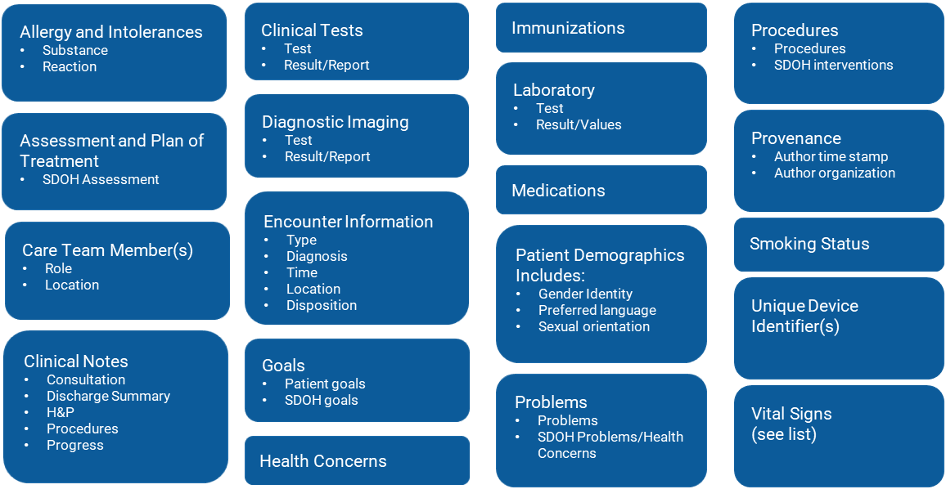
\includegraphics[width=1\linewidth]{assets/chapter_1/uscdi_v2} 

}

\caption{USCDI v2}\label{fig:uscdi}
\end{figure}

\begin{itemize}
\tightlist
\item
  \href{https:/healthit.gov/isa/uscdi-data-class}{US Core Data for Interoperability v2}
\end{itemize}

\hypertarget{fast-healthcare-interoperability-resources-fhir}{%
\subsection{Fast Healthcare Interoperability Resources (FHIR)}\label{fast-healthcare-interoperability-resources-fhir}}

\begin{itemize}
\item
  \href{https://onlinelibrary.wiley.com/doi/full/10.1002/\%20lrh2.10065}{Lehmann HP, Downs SM. Desiderata for sharable computable biomedical knowledge for learning health systems. Learn Health Syst. 2018;2(4):e10065. https://onlinelibrary.wiley.com/doi/full/10.1002/ lrh2.10065.}
\item
  \href{https://www.hl7.org/fhir/us/core/index.html}{USCDI FHIR Implementation Guide}

  \begin{itemize}
  \item
    \href{https://www.hl7.org/fhir/us/core/StructureDefinition-us-core-condition.html\#notes}{Condition Profile}
  \item
    \href{https://www.hl7.org/fhir/us/core/StructureDefinition-us-core-observation-lab.html\#mandatory-search-parameters}{Laboratory Results Reporting}
  \item
    \href{https://www.hl7.org/fhir/us/core/StructureDefinition-us-core-blood-pressure.html\#mandatory-search-parameters}{Vital Sign Profile}
  \item
    \href{https://www.hl7.org/fhir/us/core/StructureDefinition-us-core-medication.html}{Medication Profile}
  \item
    \href{https://www.hl7.org/fhir/us/core/StructureDefinition-us-core-medicationrequest.html}{MedicationRequest Profile}
  \end{itemize}
\end{itemize}

\hypertarget{common-data-models}{%
\subsection{Common Data Models}\label{common-data-models}}

\begin{itemize}
\item
  \href{https://pcornet.org/}{The National Patient-Centered Clinical Research Network (PCORnet)}

  \begin{itemize}
  \tightlist
  \item
    \href{https://pcornet.org/wp-content/uploads/2022/01/PCORnet-Common-Data-Model-v60-2020_10_221.pdf}{PCORnet Common Data Model v6.0}
  \end{itemize}
\item
  \href{https://www.ohdsi.org/}{Observational Health Data Sciences and Informatics (OHDSI)}

  \begin{itemize}
  \tightlist
  \item
    \href{https://ohdsi.github.io/TheBookOfOhdsi/}{The Book of OHDSI}
  \item
    \href{https://ohdsi.github.io/CommonDataModel/cdm53.html}{OMOP Common Data Model v5.3}
  \end{itemize}
\end{itemize}

\hypertarget{interoperable-use-cases-for-conditions-and-diagnoses}{%
\section{Interoperable Use Cases for CONDITIONS and DIAGNOSES}\label{interoperable-use-cases-for-conditions-and-diagnoses}}

This chapter provides references and resources for learning more about patient condition diagnoses.

\hypertarget{computable-phenotyping}{%
\subsection{Computable Phenotyping}\label{computable-phenotyping}}

\begin{itemize}
\tightlist
\item
  \href{https://rethinkingclinicaltrials.org/chapters/conduct/electronic-health-records-based-phenotyping/electronic-health-records-based-phenotyping-introduction/}{Electronic Health Records-Based Phenotyping}
\item
  \href{https://www.sciencedirect.com/science/article/pii/S0933365716300641?via\%3Dihub}{Richesson LR, Sun J, Pathak J, Kho AN, Denny JC. Clinical Phenotyping in selected national networsk: demonstrating the need for high-throughput, portable and computational methods. Artif Intell Med. 2016 July; 71:57-61.}
\end{itemize}

\hypertarget{terminologies}{%
\subsection{Terminologies}\label{terminologies}}

\begin{itemize}
\tightlist
\item
  \href{https://www.cms.gov/medicare/icd-10/2022-icd-10-cm}{ICD-10 CM}

  \begin{itemize}
  \tightlist
  \item
    \href{https://ftp.cdc.gov/pub/health_statistics/nchs/publications/ICD10CM/2022/icd10cm_tabular_2022.pdf}{Tabular browser view download}
  \item
    \href{https://icd10cmtool.cdc.gov/}{Alpha browsing tool}
  \item
    Available from \href{https://www.cms.gov/medicare/icd-10/2022-icd-10-cm}{CMS} or \href{https://ftp.cdc.gov/pub/Health_Statistics/NCHS/Publications/ICD10CM/2022/}{CDC}
  \end{itemize}
\item
  \href{https://www.snomed.org/}{SNOMED CT}

  \begin{itemize}
  \tightlist
  \item
    \href{https://browser.ihtsdotools.org/}{SNOMED CT Browser}
  \item
    Downloads of SNOMED International + US Extension available twice yearly (March and September) from \href{https://uts.nlm.nih.gov/uts/}{NLM terminology services}
  \end{itemize}
\end{itemize}

\hypertarget{interoperable-use-cases-for-lab-results-including-covid-19-and-anatomic-pathology}{%
\section{Interoperable Use Cases for LAB RESULTS including COVID-19 and ANATOMIC PATHOLOGY}\label{interoperable-use-cases-for-lab-results-including-covid-19-and-anatomic-pathology}}

This chapter provides references and resources for learning more about the interoperation of laboratory terminology and anaomtic pathology.

\hypertarget{loinc}{%
\subsection{LOINC}\label{loinc}}

\begin{itemize}
\tightlist
\item
  \href{https://loinc.org/}{LOINC}

  \begin{itemize}
  \tightlist
  \item
    LOINC publishes release twice annually and supports \href{https://loinc.org/search/}{downloads and browsing tools}
  \item
    Browsing and term lookup available in \href{https://loinc.org/relma/}{RELMA tool} and from the \href{https://loinc.org/search/}{LOINC website}
  \item
    Frequency analysis of US lab results from our site included in handout material: \href{https://github.com/UNMC-CRANE/AMIA_Workshop_May_2022/blob/main/Handouts/NEBRASKA_SEMANTIC_CODE_FREQUENCYfinal.xlsx}{NEBRASKA\_SEMANTIC\_CODE\_FREQUENCY.xlsx}
  \item
    Structured Terminology Model of Meaning: \href{https://github.com/UNMC-CRANE/AMIA_Workshop_May_2022/blob/main/Handouts/LOINCUsersGuide.pdf}{LOINCUsersGuide.pdf}
  \end{itemize}
\end{itemize}

\hypertarget{synoptic-pathology}{%
\subsection{Synoptic Pathology}\label{synoptic-pathology}}

\begin{itemize}
\tightlist
\item
  College of American Pathologists \href{https://www.cap.org/protocols-and-guidelines/cancer-reporting-tools/cancer-protocol-templates}{Cancer Protocol Templates}
\item
  \href{https://www.unmc.edu/pathology-research/bioinformatics/campbell/tdc.html}{Nebraska Lexicon}
\end{itemize}

\hypertarget{interoperable-use-cases-for-medication-orders-medication-administration-and-drug-allergies}{%
\section{Interoperable Use Cases for MEDICATION ORDERS, MEDICATION ADMINISTRATION and DRUG ALLERGIES}\label{interoperable-use-cases-for-medication-orders-medication-administration-and-drug-allergies}}

This chapter provides references and resources for learning more about the interoperation of medication orders, medication administration, and drug allergies.

\hypertarget{rxnorm}{%
\subsection{RxNorm}\label{rxnorm}}

\begin{itemize}
\tightlist
\item
  First published by NLM in 2002 as \href{https://www.nlm.nih.gov/research/umls/rxnorm/index.html}{UMLS project for standardized nomenclature for US clinical drugs}
\item
  Downloads available at \href{https://uts.nlm.nih.gov/uts/}{UMLS Terminology Services}
\item
  Browsing supported by \href{https://mor.nlm.nih.gov/RxNav/}{RxNav} for terms and semantic network
\item
  \href{https://lhncbc.nlm.nih.gov/RxNav/applications/RxNav-in-a-Box.html}{RxNav-in-a-Box} supports local-installable Docker version of all APIs and allows updating of all RXNorm data files
\item
  \href{https://lhncbc.nlm.nih.gov/RxNav/applications/RxClassIntro.html}{RxClass API} supports maps to drug classification schemes
\item
  Handouts: \href{https://github.com/UNMC-CRANE/AMIA_Workshop_May_2022/blob/main/Handouts/RXNORM_NDC_RELATIONSHIPS_20220501.zip}{RXNORM\_NDC\_RELATIONSHIPS\_20220501.zip}
\end{itemize}

\hypertarget{national-drug-codes-ndc}{%
\subsection{National Drug Codes (NDC)}\label{national-drug-codes-ndc}}

\begin{itemize}
\tightlist
\item
  Database maintained by the FDA and reported in \href{https://mor.nlm.nih.gov/RxNav/}{RxNav} which requires manufacturers to report all drugs manufactured, prepared, propagated, compounded or processed for sale in the US
\item
  Handouts: \href{https://github.com/UNMC-CRANE/AMIA_Workshop_May_2022/blob/main/Handouts/RXNORM_NDC_RELATIONSHIPS_20220501.zip}{RXNORM\_NDC\_RELATIONSHIPS\_20220501.zip}
\end{itemize}

\hypertarget{interoperable-use-cases-for-vitals-clinical-assessments-nursing-assessments-and-social-determinants-of-health}{%
\section{Interoperable Use Cases for VITALS, CLINICAL ASSESSMENTS, NURSING ASSESSMENTS and SOCIAL DETERMINANTS OF HEALTH}\label{interoperable-use-cases-for-vitals-clinical-assessments-nursing-assessments-and-social-determinants-of-health}}

This chapter provides references and resources for learning more about the interoperation of vitals, assessments, and social determinants of health (SDOH).

\hypertarget{assessments}{%
\section{Assessments}\label{assessments}}

\begin{itemize}
\item
  \href{https://loinc.org/}{LOINC}
\item
  \href{https://www.snomed.org/}{SNOMED CT}
  \# Social Determinants of Health (SDOH)
\item
  \href{https://health.gov/healthypeople/objectives-and-data/social-determinants-health}{Healthy People 2030}
\item
  Efforts made to standardize SDOH data elements:

  \begin{itemize}
  \tightlist
  \item
    \href{https://www.who.int/health-topics/social-determinants-of-health\#tab=tab_1}{World Health Organization}
  \item
    \href{https://thegravityproject.net/}{The Gravity Project}
  \item
    \href{https://www.healthit.gov/isa/uscdi-data-class/social-determinants-health}{USCDI}
  \item
    Research Networks

    \begin{itemize}
    \tightlist
    \item
      \href{https://github.com/OHDSI/HealthEquityWG}{OHDSI Health Equity Workgroup}
    \item
      \href{https://covid.cd2h.org/social-determinants}{N3C SDOH Domain Team}
    \end{itemize}
  \item
    Regional and National Measures and Indices

    \begin{itemize}
    \tightlist
    \item
      US Census \href{https://www.census.gov/programs-surveys/acs}{American Community Survey}
    \item
      Wisconsin \href{https://www.neighborhoodatlas.medicine.wisc.edu/}{Area Deprivation Index}
    \item
      CDC \href{https://www.atsdr.cdc.gov/placeandhealth/svi/index.html}{Social Vulnerability Index}
    \item
      \href{https://www.ncbi.nlm.nih.gov/pmc/articles/PMC3432399/}{BIRD Index}
    \item
      USDA ERS \href{https://www.ers.usda.gov/data-products/rural-urban-commuting-area-codes/documentation/}{Rural Urban Commuting Area (RUCA) Codes}
    \item
      USDA \href{https://www.ers.usda.gov/data-products/food-environment-atlas/}{Food Environment Atlas}
    \end{itemize}
  \end{itemize}
\end{itemize}

\hypertarget{references}{%
\section{References}\label{references}}

\textbf{Selected references from this workhop include:}

\begin{enumerate}
\def\labelenumi{\arabic{enumi}.}
\tightlist
\item
  The Learning Healthcare System. Ed: LeeAnne Olsen, Dara Aisner, Michael McGinnis. Institute of Medicine, National Academy of Sciences 2007
\item
  Lehmann HP, Downs SM. Desiderata for sharable computable biomedical knowledge for learning health systems. Learn Health Syst. 2018;2(4):e10065. \url{https://onlinelibrary.wiley.com/doi/full/10.1002/} lrh2.10065.
\item
  OHDSI. The Book of OHDSI: Observational Health Data Sciences and Informatics. OHDSI; 2021.
\item
  Yu Y, Zong N, Wen A, et al.~Developing an ETL tool for converting the PCORnet CDM into the OMOP CDM to facilitate the COVID-19 data integration.~J Biomed Inform. 2022;127:104002. \url{doi:10.1016/j.jbi.2022.104002}
\item
  Richesson LR, Sun J, Pathak J, Kho AN, Denny JC. Clinical Phenotyping in selected national networsk: demonstrating the need for high-throughput, portable and computational methods. Artif Intell Med. 2016 July; 71:57-61.
\item
  Cimino-J. Desiderata for Controlled Medical Vocabularies in the Twenty-First Century. Methods Information in Medicine. 1998 Nov; 37(4-5):394-403.
\item
  Bodenreider O, Cornet R, Vreeman DJ. Recent developments in clinical terminologies SNOMED CT, LOINC and RxNorm. Yearbook Med Inform 2018;27(1):129-139.
\item
  Teasdale G, Jennett B. Assessment of coma and impaired consciousness. Lancet 1974; 81-84.
\item
  Teasdale G, Jennett B. Assessment and prognosis of coma after head injury. Acta Neurochir 1976; 34:45-55.
\item
  Westra, Bonnie L., et al.~``Validation and refinement of a pain information model from EHR flowsheet data.'' Applied clinical informatics. 9.01 (2018): 185-198.
\item
  Healthy People 2030, U.S. Department of Health and Human Services, Office of Disease Prevention and Health Promotion. Retrieved {[}08 May 2022{]}, from \url{https://health.gov/healthypeople/objectives-and-data/social-determinants-health}
\item
  McClure et al.~Gender harmony: improved standards to support affirmative care of gender-marginalized people through inclusive gender and sex representation {[}published correction appears in J Am Med Inform Assoc. 2021 Nov 25;:{]}. J Am Med Inform Assoc. 2022;29(2):354-363. \url{doi:10.1093/jamia/ocab196}
\end{enumerate}

  \bibliography{book.bib,packages.bib}

\end{document}
